\documentclass{article}
    % General document formatting
    \usepackage[margin=0.7in]{geometry}
    \usepackage[parfill]{parskip}
    \usepackage[utf8]{inputenc}
    
    % Related to math
    \usepackage{amsmath,amssymb,amsfonts,amsthm}
\usepackage{tikz}
\usepackage{subfigure}
\usetikzlibrary{bayesnet}

\begin{document}


\begin{figure}[ht]
\begin{center}
\begin{tabular}{cc}
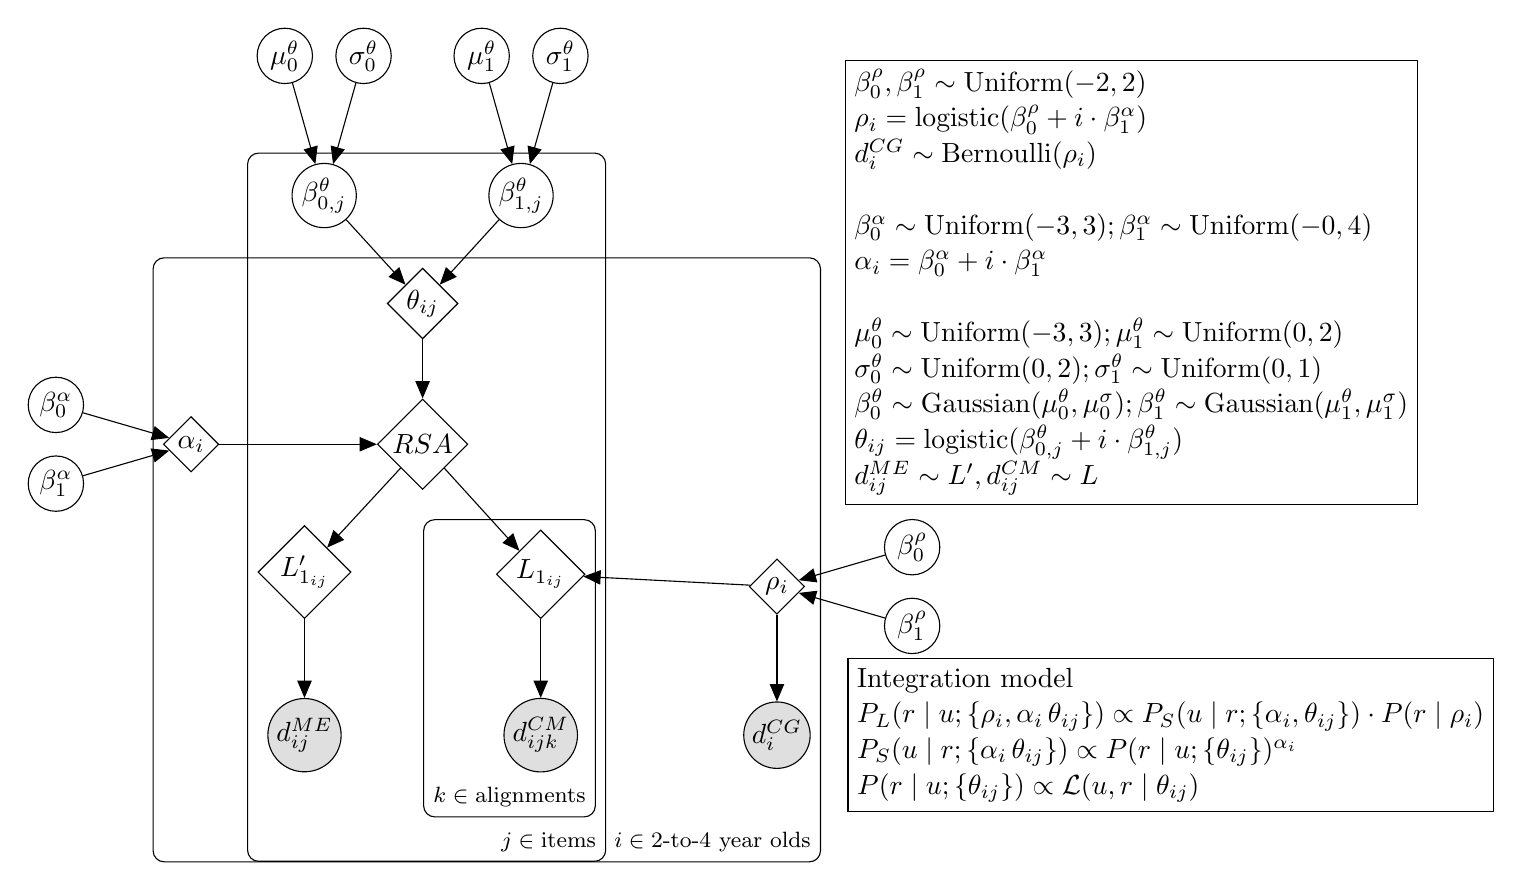
\begin{tikzpicture}
%% RSA nodes and data
\node[obs](data_comb){$d^{CM}_{ijk}$};
\node[obs, xshift=-3cm, yshift=0cm](data_me){$d^{ME}_{ij}$};
\node[obs, xshift=3cm,  yshift=0cm](data_cg){$d^{CG}_{i}$};

\node[det, above=of data_me](L1_me){$L'_{1_{ij}}$};
\node[det, above=of data_comb](L1_comb){$L_{1_{ij}}$};
\node[det, above=of L1_comb, xshift=-1.5cm, yshift=-0.5cm](RSA){$RSA$};

\edge{L1_me}{data_me};
\edge{L1_comb}{data_comb};
\edge{RSA}{L1_me};
\edge{RSA}{L1_comb};

% COMMON GROUND
\node[det, above=of data_cg, yshift=0.1cm](rho){$\rho_i$};
\node[latent, right=of rho, yshift=0.5cm](beta_rho_int){$\beta^{\rho}_0$};
\node[latent, right=of rho, yshift=-0.5cm](beta_rho_slope){$\beta^{\rho}_1$};

\edge{rho}{data_cg};
\edge{beta_rho_int}{rho};
\edge{beta_rho_slope}{rho};
\edge{rho}{L1_comb};

%% SPEAKER INFORMATIVITY

\node[det, left=of RSA, xshift=-1cm](alpha){$\alpha_i$};
\node[latent, left=of alpha, yshift=0.5cm](beta_alpha_int){$\beta^{\alpha}_0$};
\node[latent, left=of alpha, yshift=-0.5cm](beta_alpha_slope){$\beta^{\alpha}_1$};

%	\edge{alpha}{L1_me};
\edge{beta_alpha_int}{alpha};
\edge{beta_alpha_slope}{alpha};
\edge{alpha}{RSA};

%% SEMANTIC KNOWLEDGE model

	\node[det, above=of RSA, yshift=-0.25cm](theta){$\theta_{ij}$};
\node[latent, above=of theta, xshift=-1.25cm, yshift=-0.5cm](beta_theta_int){$\beta^{\theta}_{0, j}$};
\node[latent, above=of theta, xshift=1.25cm, yshift=-0.5cm](beta_theta_slope){$\beta^{\theta}_{1, j}$};

\node[latent, above=of beta_theta_int, xshift=-0.5cm](mu_theta_int){$\mu^{\theta}_{0}$};
\node[latent, above=of beta_theta_int, xshift=0.5cm](sigma_theta_int){$\sigma^{\theta}_{0}$};

\node[latent, above=of beta_theta_slope, xshift=-0.5cm](mu_theta_slope){$\mu^{\theta}_{1}$};
\node[latent, above=of beta_theta_slope, xshift=0.5cm](sigma_theta_slope){$\sigma^{\theta}_{1}$};

\edge{theta}{RSA};
%	\edge{theta}{L1_comb};
\edge{beta_theta_int}{theta};
\edge{beta_theta_slope}{theta};
\edge{mu_theta_int}{beta_theta_int};
\edge{sigma_theta_int}{beta_theta_int};
\edge{mu_theta_slope}{beta_theta_slope};
\edge{sigma_theta_slope}{beta_theta_slope};

\

\plate{plate_condition}{(data_comb)(L1_comb)}{$k \in \text{alignments}$};

	\plate{plate_items}{
%		(plate_data_me)
%		(plate_data_comb)
%		(plate_condition)
(plate_condition)
	(data_comb)
	(data_me)
	(L1_me)
	(L1_comb)
	(theta)
	(beta_theta_int)
	(beta_theta_slope)
}{$j \in \text{items}$}

	\plate{plate_data_comb}{
	(data_comb)
	(data_cg)
	(data_me)
	(plate_condition)
	(rho)
	(theta)
	(alpha)
	(L1_me)
	(L1_comb)
%		(plate_items)
	}{$i \in \text{2-to-4 year olds}$}



\node[draw, align=left, execute at begin node=\setlength{\baselineskip}{3ex}] at (7.5,5.75) { 
$\beta^\rho_0 ,\beta^\rho_1 \sim \text{Uniform}(-2,2)$ \\
 $\rho_i = \text{logistic}(\beta^\rho_0  + i \cdot \beta^\alpha_1)$ \\
 $d^{CG}_{i} \sim \text{Bernoulli}(\rho_i)$ \\
 \\
$\beta^\alpha_0 \sim \text{Uniform}(-3,3); \beta^\alpha_1 \sim \text{Uniform}(-0,4)$ \\
 $\alpha_i = \beta^\alpha_0  + i \cdot \beta^\alpha_1$ \\
 \\
 $\mu^\theta_0 \sim \text{Uniform}(-3,3); \mu^\theta_1 \sim \text{Uniform}(0,2)$ \\
 $\sigma^\theta_0 \sim \text{Uniform}(0,2); \sigma^\theta_1 \sim \text{Uniform}(0,1)$ \\
 $\beta^\theta_0 \sim \text{Gaussian}(\mu^\theta_0, \mu^\sigma_0); \beta^\theta_1 \sim \text{Gaussian}(\mu^\theta_1, \mu^\sigma_1)$  \\
 $\theta_{ij} = \text{logistic}(\beta^\theta_{0,j}  + i \cdot \beta^\theta_{1,j})$ \\
 $d^{ME}_{ij} \sim L',  d^{CM}_{ij} \sim L$
};

\node[draw, align=left, execute at begin node=\setlength{\baselineskip}{3ex}] at (8,0) {Integration model\\ $P_{L}(r \mid u; \{\rho_i, \alpha_i\, \theta_{ij}\})\propto P_{S}(u \mid r; \{\alpha_i, \theta_{ij}\}) \cdot P(r \mid \rho_i) $\\ 
$P_{S}(u \mid r; \{\alpha_i\, \theta_{ij}\})\propto P(r \mid u; \{\theta_{ij}\}) ^{\alpha_i} $\\
$P(r \mid u; \{\theta_{ij}\}) \propto \mathcal{L}(u, r \mid \theta_{ij})$
};


\end{tikzpicture}

    \end{tabular}
  \end{center}
  \caption{Graphical model representing the Bayesian data analysis for \emph{Integration model} used for \emph{Explanation}. $L$ represents the RSA model defined by Eq. X, used to predict the Combination Data $d^{CM}$  from Expt.~3 for each unique age bin $i$, lexical item $j$, and alignment condition $k$. This RSA model takes as input a speaker optimality parameter $\alpha_i$ (which varies by age), a semantic knowledge parameter $\theta_{ij}$ (which varies by age and item), and a common ground sensitivity $\rho_i$ (which varies by age). Speaker optimality and semantic knowledge parameters are additionally constrained by the data from the Mutual Exclusivity task ($d^{ME}$; Expt.~1), via the same RSA model with no common ground $L$;  common ground sensitivity parameters $\rho_i$ are directly constrained by the data from the Common Ground experiment ($d^{CG}$; Expt.~2).  
  Each of these RSA parameters is sampled from a linear or logistic regression model that track developmental change (with intercepts and slopes given by $\beta_0$ and $\beta_1$, respectively). Additionally, the semantic knowledge parameters for individual items $j$ are sampled from global vocabulary developmental parameters $\mu$ and $\sigma$ that characterize the mean and standard deviation of the intercepts and slopes for individual item trajectories.}
  \label{fig:bayesnet}
\end{figure}
%S2 represents the RSA speaker model defined by Eq. 1, which is used to predict the production responses dprod of each participant i, for each state s (number of hearts), for each utterance w, in each goal condition g. The RSA speaker model takes as input the literal meaning variables θ, which additionally are used to predict the literal meaning judgments dlit assuming a Bernoulli linking function. Additionally, the RSA model takes the speaker’s goal weights ω and intended presentational goal weight φ, which are inferred separately for each goal condition g. Finally, the RSA model uses two global free parameters: the cost of negation c and the speaker’s rationality parameter α.


\begin{figure}[ht]
\begin{center}
\begin{tabular}{cc}
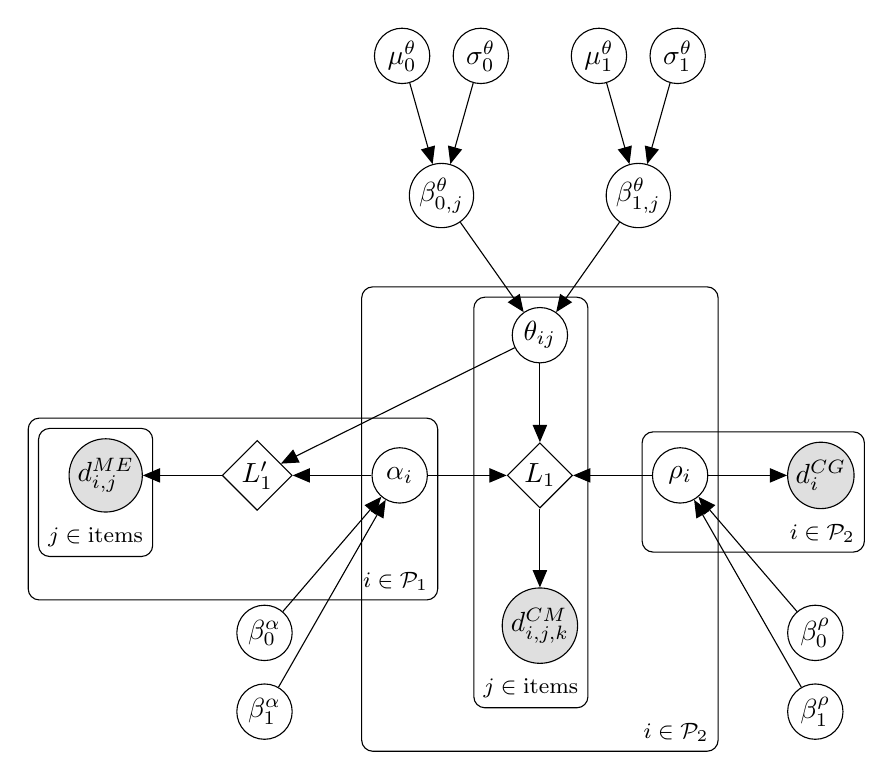
\begin{tikzpicture}
	%% RSA nodes and data
	\node[obs](data_comb){$d^{CM}_{i, j, k}$};
	\node[det, above=of data_comb](L1_comb){$L_1$};
	\edge{L1_comb}{data_comb};

	
%	\node[det, right=of data_me](L1_me){$L'_1$};
	
%	\edge{L1_me}{data_me};
	
	% COMMON GROUND
	\node[latent, right=of L1_comb](rho){$\rho_i$};
	\node[obs, right=of rho](data_cg){$d^{CG}_{i}$};
	\node[latent, right=of rho, yshift=-2cm](beta_rho_int){$\beta^{\rho}_0$};
	\node[latent, right=of rho, yshift=-3cm](beta_rho_slope){$\beta^{\rho}_1$};
	
	\edge{rho}{data_cg};
	\edge{beta_rho_int}{rho};
	\edge{beta_rho_slope}{rho};
	\edge{rho}{L1_comb};
	
	%% SPEAKER INFORMATIVITY
	
	\node[latent, left=of L1_comb](alpha){$\alpha_i$};
	\node[latent, left=of alpha, yshift=-2cm](beta_alpha_int){$\beta^{\alpha}_0$};
	\node[latent, left=of alpha, yshift=-3cm](beta_alpha_slope){$\beta^{\alpha}_1$};
	\node[det, left=of alpha](L1_me){$L'_1$};
	\node[obs, left=of L1_me](data_me){$d^{ME}_{i, j}$};

	\edge{alpha}{L1_me};
	\edge{beta_alpha_int}{alpha};
	\edge{beta_alpha_slope}{alpha};
	\edge{alpha}{L1_comb};
	\edge{L1_me}{data_me};
	
	%% SEMANTIC KNOWLEDGE model

	\node[latent, above=of L1_comb](theta){$\theta_{ij}$};
	\node[latent, above=of theta, xshift=-1.25cm](beta_theta_int){$\beta^{\theta}_{0, j}$};
	\node[latent, above=of theta, xshift=1.25cm](beta_theta_slope){$\beta^{\theta}_{1, j}$};
	
	\node[latent, above=of beta_theta_int, xshift=-0.5cm](mu_theta_int){$\mu^{\theta}_{0}$};
	\node[latent, above=of beta_theta_int, xshift=0.5cm](sigma_theta_int){$\sigma^{\theta}_{0}$};
	
	\node[latent, above=of beta_theta_slope, xshift=-0.5cm](mu_theta_slope){$\mu^{\theta}_{1}$};
	\node[latent, above=of beta_theta_slope, xshift=0.5cm](sigma_theta_slope){$\sigma^{\theta}_{1}$};
	
	\edge{theta}{L1_me};
	\edge{theta}{L1_comb};
	\edge{beta_theta_int}{theta};
	\edge{beta_theta_slope}{theta};
	\edge{mu_theta_int}{beta_theta_int};
	\edge{sigma_theta_int}{beta_theta_int};
	\edge{mu_theta_slope}{beta_theta_slope};
	\edge{sigma_theta_slope}{beta_theta_slope};
	
		\plate{plate_items_me}{
		(data_me)
	}{$j \in \text{items}$}	
	
	
	\plate{plate_data_me}{
		(data_me)
		(L1_me)
		(alpha)
		(plate_items_me)
	}{$i \in \mathcal{P}_{1}$}
	

	\plate{plate_data_cg}{
		(data_cg)(rho)
	}{$i \in \mathcal{P}_{2}$}
	
	\plate{plate_items}{
		(data_comb)(L1_comb)(theta)
	}{$j \in \text{items}$}	
	
	\plate{plate_data_comb}{
		(data_comb)(rho)(alpha)(theta)(plate_items)
	}{$i \in \mathcal{P}_{2}$}



\end{tikzpicture}

    \end{tabular}
  \end{center}
  \caption{ Put a caption here.}
  \label{fig:bayesnet}
\end{figure}

\begin{figure}[ht]
\begin{center}
\begin{tabular}{cc}
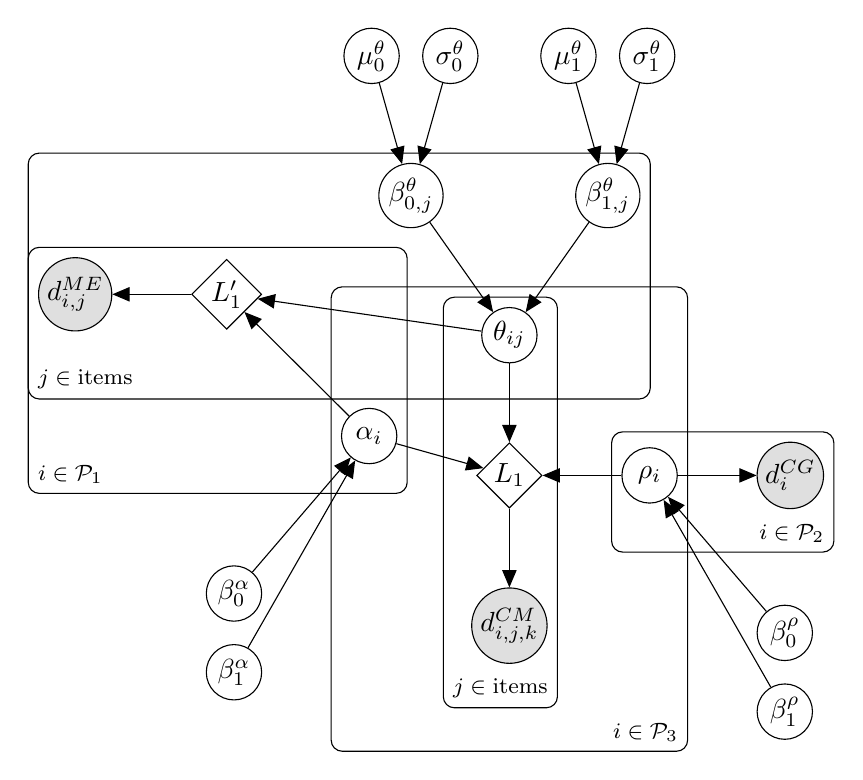
\begin{tikzpicture}
	%% RSA nodes and data
	\node[obs](data_comb){$d^{CM}_{i, j, k}$};
	\node[det, above=of data_comb](L1_comb){$L_1$};
	\edge{L1_comb}{data_comb};

	
%	\node[det, right=of data_me](L1_me){$L'_1$};
	
%	\edge{L1_me}{data_me};
	
	% COMMON GROUND
	\node[latent, right=of L1_comb](rho){$\rho_i$};
	\node[obs, right=of rho](data_cg){$d^{CG}_{i}$};
	\node[latent, right=of rho, yshift=-2cm](beta_rho_int){$\beta^{\rho}_0$};
	\node[latent, right=of rho, yshift=-3cm](beta_rho_slope){$\beta^{\rho}_1$};
	
	\edge{rho}{data_cg};
	\edge{beta_rho_int}{rho};
	\edge{beta_rho_slope}{rho};
	\edge{rho}{L1_comb};
	
	%% SPEAKER INFORMATIVITY
	
	\node[latent, left=of L1_comb, yshift=0.5cm](alpha){$\alpha_i$};
	\node[latent, left=of alpha, yshift=-2cm](beta_alpha_int){$\beta^{\alpha}_0$};
	\node[latent, left=of alpha, yshift=-3cm](beta_alpha_slope){$\beta^{\alpha}_1$};
	\node[det, left=of alpha, yshift=1.8cm](L1_me){$L'_1$};
	\node[obs, left=of L1_me](data_me){$d^{ME}_{i, j}$};

	\edge{alpha}{L1_me};
	\edge{beta_alpha_int}{alpha};
	\edge{beta_alpha_slope}{alpha};
	\edge{alpha}{L1_comb};
	\edge{L1_me}{data_me};
	
	%% SEMANTIC KNOWLEDGE model

	\node[latent, above=of L1_comb](theta){$\theta_{ij}$};
	\node[latent, above=of theta, xshift=-1.25cm](beta_theta_int){$\beta^{\theta}_{0, j}$};
	\node[latent, above=of theta, xshift=1.25cm](beta_theta_slope){$\beta^{\theta}_{1, j}$};
	
	\node[latent, above=of beta_theta_int, xshift=-0.5cm](mu_theta_int){$\mu^{\theta}_{0}$};
	\node[latent, above=of beta_theta_int, xshift=0.5cm](sigma_theta_int){$\sigma^{\theta}_{0}$};
	
	\node[latent, above=of beta_theta_slope, xshift=-0.5cm](mu_theta_slope){$\mu^{\theta}_{1}$};
	\node[latent, above=of beta_theta_slope, xshift=0.5cm](sigma_theta_slope){$\sigma^{\theta}_{1}$};
	
	\edge{theta}{L1_me};
	\edge{theta}{L1_comb};
	\edge{beta_theta_int}{theta};
	\edge{beta_theta_slope}{theta};
	\edge{mu_theta_int}{beta_theta_int};
	\edge{sigma_theta_int}{beta_theta_int};
	\edge{mu_theta_slope}{beta_theta_slope};
	\edge{sigma_theta_slope}{beta_theta_slope};
	
	{
	\tikzset{plate caption/.append style={below right=2pt and 0pt of #1.south west}}
		\plate{plate_items_me}{
			(data_me)(L1_me)(theta)(beta_theta_int)(beta_theta_slope)
		}{$j \in \text{items}$}	
	}
	
	{
	\tikzset{plate caption/.append style={below right=0pt and 0pt of #1.south west}}
	\plate{plate_data_me}{
		(data_me)
		(L1_me)
		(alpha)
%		(plate_items_me)
	}{$i \in \mathcal{P}_{1}$}
	}

	\plate{plate_data_cg}{
		(data_cg)(rho)
	}{$i \in \mathcal{P}_{2}$}
	
	\plate{plate_items}{
		(data_comb)(L1_comb)(theta)
	}{$j \in \text{items}$}	
	
	\plate{plate_data_comb}{
		(data_comb)(rho)(alpha)(theta)(plate_items)
	}{$i \in \mathcal{P}_{3}$}



\end{tikzpicture}

    \end{tabular}
  \end{center}
  \caption{ Put a caption here.}
  \label{fig:bayesnet}
\end{figure}




\end{document}

